\documentclass[floatfix,prb,aps,superscriptaddress,11pt,preprint,letterpaper]{revtex4}
\usepackage{amsfonts}
\usepackage{amsmath}
\usepackage{graphicx}
\allowdisplaybreaks[1]%biutiful equation breaker!!!
\usepackage{ulem}
\usepackage{subfigure}
\usepackage{bm}
%%%%*****************%%%% fine hyperef 
\usepackage[backref,pdffitwindow,colorlinks,linkcolor={blue},citecolor={red}]{hyperref}
%%%%%%%%%%%%%%%%%%%%%%%%%%%%%%%%%%%%%%%
\usepackage{showlabels}
\pagestyle{empty}
%\usepackage{showkeys}

\begin{document}
%%%%%%%%%%%%%%%%%%%%%%%%%%%%%%
\begin{center}
Si(001)$2\times 1$ reconstruction\\
$\chi^{xxx}_{\mathrm{2\times 1}}\ne 0$\\
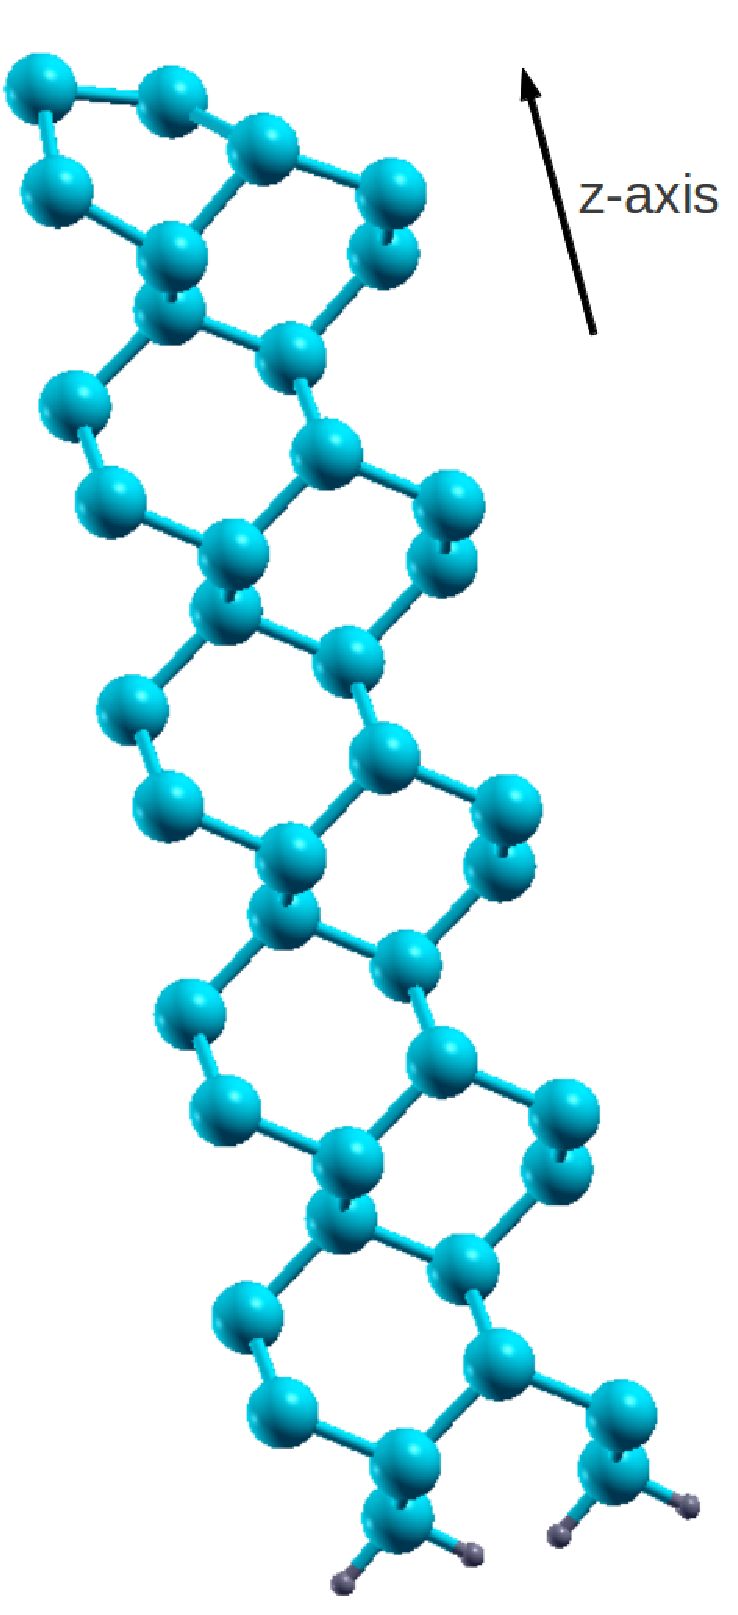
\includegraphics[scale=.25]{AsymDiHz}\\
H-terminated $\Rightarrow\chi^{xxx}_{\mathrm{H}}= 0$
\begin{picture}(5,20) 
\put(-140,110){\line(1,0){150}}
\put(-150,160){$\textcolor{red}{{\cal C}^\ell(z)}=1$}
\put(-150,60){$\textcolor{red}{{\cal C}^\ell(z)}=0$}
\end{picture}
\end{center}
%%%%%%%%%%%%%%%%%%%%%%%%%%%%%%
\end{document}
